\section{Exercise 5: Kullback-Leibler divergence from empirical distribution}

\begin{frame}{Kullback-Leibler divergence}
	
	In this exercise we try to identify which binomial distribution is the best analytical fit for our sampled distribution.
	
	To do so, we need to introduce the concept of \textbf{Kullback-Leibler divergence}. Kullback-Leibler divergence is a statistical measure that quantifies how much one probability distribution differs from a second, reference probability distribution. KL divergence is closely linked to conditional entropy and information gain, because it measures how much more uncertainty is introduced by using one probability distribution instead of another.
	
	For two probability distributions \(P\) (the observed distribution) and \(Q\) (the analytical fit), the KL divergence from \(Q\) to \(P\) is given by:
	
	\[
	D_{KL}(P || Q) = \sum_{x} P(x) \log \left( \frac{P(x)}{Q(x)} \right)
	\]
	
\end{frame}

\begin{frame}{Observed Distribution}
	Consider the following observed data:
	
	\[
	x_{i} = (0\quad 1\quad 2\quad 3\quad 4\quad 5\quad 6\quad 7\quad 8\quad 9\quad 10)
	\]
	
	\[
	\# \quad observed \quad x_{i} = (1\quad 3\quad 2\quad 8\quad 18\quad 41\quad 47\quad 39\quad 24\quad 8\quad 3)
	\]
	
\end{frame}

\begin{frame}{Divergence from Uniform Distribution}
	
	We compute the KL divergence of the observed distribution from a uniform distribution, to measure how distant the two probability distributions are.
	
	\begin{figure}[h]
		\centering
		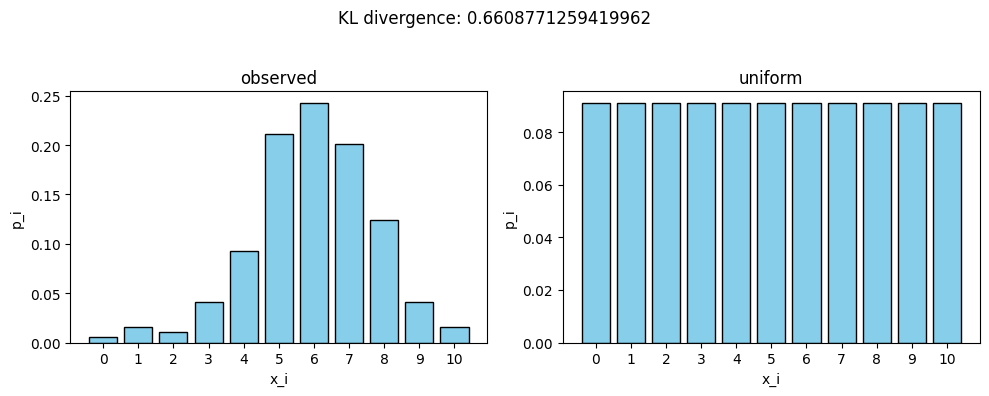
\includegraphics[width=.9\textwidth]{images/ex5/uniform_div.png}
	\end{figure}
	
\end{frame}

\begin{frame}{Search of the optimal Binomial Distribution}
	
	To find the binomial distribution closest to the observed distribution, we compute the KL divergence from each binomial distribution given \(n=11\) independent experiments and probability of success \(p\) ranging between 0 and 1 (step = 0.001).
	
	\begin{figure}[h]
		\centering
		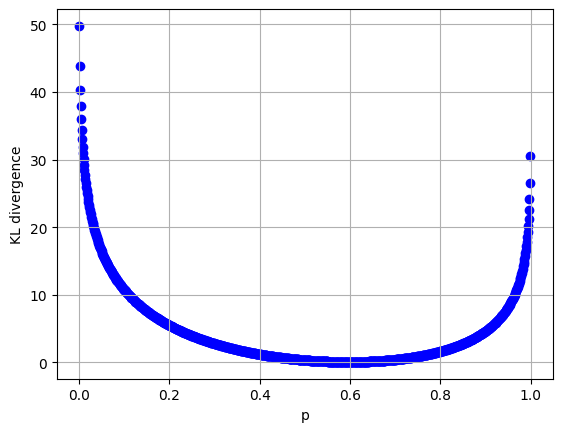
\includegraphics[width=.43\textwidth]{images/ex5/binomial_kl.png}
	\end{figure}
	
\end{frame}

\begin{frame}{Best Binomial Distribution}
	
	By minimizing the KL divergence, we determine that the optimal binomial distribution has a success probability \(p = 0.596\). We can see from the histograms that the 2 distributions are very similar and the KL divergence value has dropped significantly. 
	
	\begin{figure}[h]
		\centering
		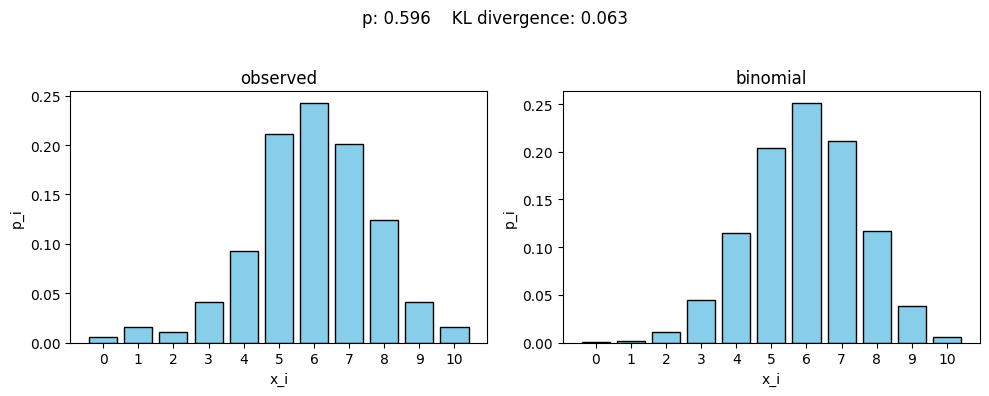
\includegraphics[width=.75\textwidth]{images/ex5/best_binomial.png}
	\end{figure}
	
\end{frame}


\begin{frame}{Conclusion}
	
	We successfully used Kullback-Leibler divergence to identify the binomial distribution that best approximates the observed data, minimizing the error committed. With this approach we can accurately model empirical distributions and also understand the degree of divergence between the observed distributions and their analytical fits.
	
\end{frame}
